%%%%%%%%%%%%%%%%%%%%%%%%%%%%%%%%%%%%%%%%%
% Thin Sectioned Essay
% LaTeX Template
% Version 1.0 (3/8/13)
%
% This template has been downloaded from:
% http://www.LaTeXTemplates.com
%
% Original Author:
% Nicolas Diaz (nsdiaz@uc.cl) with extensive modifications by:
% Vel (vel@latextemplates.com)
%
% License:
% CC BY-NC-SA 3.0 (http://creativecommons.org/licenses/by-nc-sa/3.0/)
%
%%%%%%%%%%%%%%%%%%%%%%%%%%%%%%%%%%%%%%%%%

%----------------------------------------------------------------------------------------
%	PACKAGES AND OTHER DOCUMENT CONFIGURATIONS
%----------------------------------------------------------------------------------------

\documentclass[a4paper, 11pt]{article} % Font size (can be 10pt, 11pt or 12pt) and paper size (remove a4paper for US letter paper)
\usepackage{color}
\usepackage[protrusion=true,expansion=true]{microtype} % Better typography
\usepackage{graphicx} % Required for including pictures
\usepackage{wrapfig} % Allows in-line images
\usepackage{endnotes}
\usepackage{mathpazo} % Use the Palatino font
\usepackage[T1]{fontenc} % Required for accented characters
\linespread{1.05} % Change line spacing here, Palatino benefits from a slight increase by default
\usepackage{fancyhdr}
\usepackage[margin=1.25in]{geometry}
\pagestyle{fancy}
\fancyhf{}
\rhead{Machine Learning Problem Set 3, 28.02.2019}
\lhead{Felix Adam}
\rfoot{Page \thepage}
\usepackage{amsmath}
\usepackage{amssymb}
\usepackage{version}
\usepackage{setspace}
\usepackage{enumerate}
\usepackage{multicol}
\usepackage{amsfonts}
\usepackage{amssymb}
\usepackage{subcaption,graphicx}
\usepackage{rotating}
\usepackage{lscape}
\usepackage{pdflscape}
\usepackage{array,tabularx,float,dcolumn,lscape}
\usepackage{booktabs}
\usepackage{xr}
\usepackage{dcolumn}
\usepackage{hyperref} 
\usepackage{amsmath}
\usepackage{algorithm}
\usepackage{tikz}
\usepackage[noend]{algpseudocode}
\graphicspath{ {../01_Figures/} }
\tikzset{every picture/.style={line width=0.75pt}} %set default line width to 0.75pt     


\makeatletter
\def\BState{\State\hskip-\ALG@thistlm}
\makeatother

\newlength\tindent
\setlength{\tindent}{\parindent}
\setlength{\parindent}{0pt}
\renewcommand{\indent}{\hspace*{\tindent}}
\renewcommand{\familydefault}{\sfdefault}

\makeatletter
\renewcommand\@biblabel[1]{\textbf{#1.}} % Change the square brackets for each bibliography item from '[1]' to '1.'
\renewcommand{\@listI}{\itemsep=0pt} % Reduce the space between items in the itemize and enumerate environments and the bibliography

\renewcommand{\maketitle}{ % Customize the title - do not edit title and author name here, see the TITLE block below
\begin{flushright} % Right align
{\LARGE\@title} % Increase the font size of the title

\vspace{50pt} % Some vertical space between the title and author name

{\large\@author} % Author name
\\\@date % Date

\vspace{40pt} % Some vertical space between the author block and abstract
\end{flushright}
}

\begin{document}

\section*{VC-Dimension of Circles}

For the first part of the question, we need to determine the VC-Dimension of the class $\mathcal{A}$ of all circles in $R^2$, without any restrictions on the radius. 

$$ \mathcal { A } = \left\{ C _ { \boldsymbol { c } , r } : \boldsymbol { c } \in \mathbb { R } ^ { 2 } , r \geq 0 \right\}$$

Clearly, one point can always be shattered by a circle, since it's either in or out of it. The same holds for two points. Three points can also be shattered, seen in the following: \\

\tikzset{every picture/.style={line width=0.75pt}} %set default line width to 0.75pt        

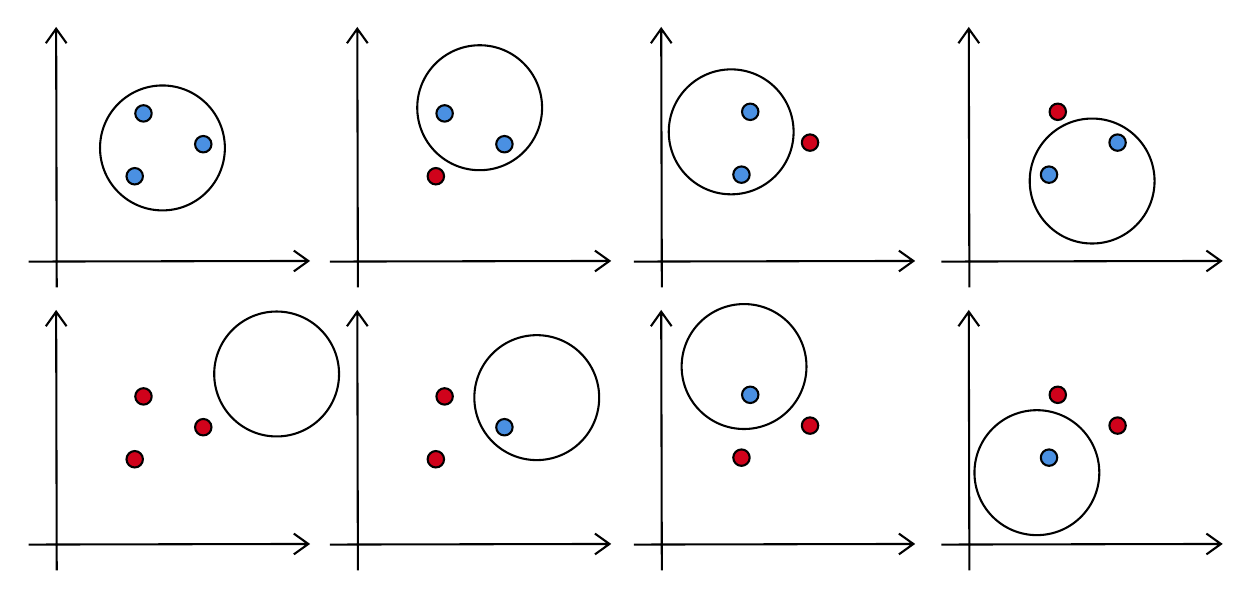
\begin{tikzpicture}[x=0.75pt,y=0.75pt,yscale=-1,xscale=1]
%uncomment if require: \path (0,414); %set diagram left start at 0, and has height of 414

%Shape: Ellipse [id:dp7692124746801012] 
\draw   (29.41,72.43) .. controls (29.41,55.8) and (42.88,42.33) .. (59.49,42.33) .. controls (76.09,42.33) and (89.56,55.8) .. (89.56,72.43) .. controls (89.56,89.05) and (76.09,102.53) .. (59.49,102.53) .. controls (42.88,102.53) and (29.41,89.05) .. (29.41,72.43) -- cycle ;
%Shape: Ellipse [id:dp8126653472568731] 
\draw  [fill={rgb, 255:red, 74; green, 144; blue, 226 }  ,fill opacity=1 ] (46.38,55.79) .. controls (46.38,53.61) and (48.15,51.83) .. (50.34,51.83) .. controls (52.53,51.83) and (54.3,53.61) .. (54.3,55.79) .. controls (54.3,57.98) and (52.53,59.76) .. (50.34,59.76) .. controls (48.15,59.76) and (46.38,57.98) .. (46.38,55.79) -- cycle ;
%Shape: Ellipse [id:dp7933731782074234] 
\draw  [fill={rgb, 255:red, 74; green, 144; blue, 226 }  ,fill opacity=1 ] (42.16,86.07) .. controls (42.16,83.88) and (43.93,82.11) .. (46.12,82.11) .. controls (48.3,82.11) and (50.08,83.88) .. (50.08,86.07) .. controls (50.08,88.26) and (48.3,90.03) .. (46.12,90.03) .. controls (43.93,90.03) and (42.16,88.26) .. (42.16,86.07) -- cycle ;
%Shape: Axis 2D [id:dp5790207644361977] 
\draw  (-4.95,127.19) -- (129.77,126.88)(8.27,14.99) -- (8.55,139.62) (122.76,121.9) -- (129.77,126.88) -- (122.78,131.9) (3.29,22) -- (8.27,14.99) -- (13.29,21.98)  ;
%Shape: Ellipse [id:dp6470818868586241] 
\draw  [fill={rgb, 255:red, 74; green, 144; blue, 226 }  ,fill opacity=1 ] (75.19,70.64) .. controls (75.19,68.45) and (76.96,66.68) .. (79.14,66.67) .. controls (81.33,66.67) and (83.1,68.43) .. (83.11,70.62) .. controls (83.11,72.81) and (81.35,74.59) .. (79.16,74.59) .. controls (76.98,74.6) and (75.2,72.83) .. (75.19,70.64) -- cycle ;

%Shape: Ellipse [id:dp1779573666947204] 
\draw   (182.24,53.06) .. controls (182.24,36.43) and (195.71,22.95) .. (212.32,22.95) .. controls (228.93,22.95) and (242.39,36.43) .. (242.39,53.06) .. controls (242.39,69.68) and (228.93,83.16) .. (212.32,83.16) .. controls (195.71,83.16) and (182.24,69.68) .. (182.24,53.06) -- cycle ;
%Shape: Ellipse [id:dp7563887452502578] 
\draw  [fill={rgb, 255:red, 74; green, 144; blue, 226 }  ,fill opacity=1 ] (191.47,55.79) .. controls (191.47,53.61) and (193.25,51.83) .. (195.43,51.83) .. controls (197.62,51.83) and (199.39,53.61) .. (199.39,55.79) .. controls (199.39,57.98) and (197.62,59.76) .. (195.43,59.76) .. controls (193.25,59.76) and (191.47,57.98) .. (191.47,55.79) -- cycle ;
%Shape: Ellipse [id:dp4875580502334238] 
\draw  [fill={rgb, 255:red, 208; green, 2; blue, 27 }  ,fill opacity=1 ] (187.25,86.07) .. controls (187.25,83.88) and (189.03,82.11) .. (191.21,82.11) .. controls (193.4,82.11) and (195.17,83.88) .. (195.17,86.07) .. controls (195.17,88.26) and (193.4,90.03) .. (191.21,90.03) .. controls (189.03,90.03) and (187.25,88.26) .. (187.25,86.07) -- cycle ;
%Shape: Axis 2D [id:dp05005340019360127] 
\draw  (140.15,127.19) -- (274.86,126.88)(153.36,14.99) -- (153.65,139.62) (267.85,121.9) -- (274.86,126.88) -- (267.87,131.9) (148.38,22) -- (153.36,14.99) -- (158.38,21.98)  ;
%Shape: Ellipse [id:dp19641746569519114] 
\draw  [fill={rgb, 255:red, 74; green, 144; blue, 226 }  ,fill opacity=1 ] (220.29,70.64) .. controls (220.28,68.45) and (222.05,66.68) .. (224.23,66.67) .. controls (226.42,66.67) and (228.2,68.43) .. (228.2,70.62) .. controls (228.21,72.81) and (226.44,74.59) .. (224.25,74.59) .. controls (222.07,74.6) and (220.29,72.83) .. (220.29,70.64) -- cycle ;

%Shape: Ellipse [id:dp7584936550754144] 
\draw   (303.42,64.68) .. controls (303.42,48.06) and (316.88,34.58) .. (333.49,34.58) .. controls (350.1,34.58) and (363.57,48.06) .. (363.57,64.68) .. controls (363.57,81.3) and (350.1,94.78) .. (333.49,94.78) .. controls (316.88,94.78) and (303.42,81.3) .. (303.42,64.68) -- cycle ;
%Shape: Ellipse [id:dp9097772767445158] 
\draw  [fill={rgb, 255:red, 74; green, 144; blue, 226 }  ,fill opacity=1 ] (338.72,55.02) .. controls (338.72,52.83) and (340.49,51.06) .. (342.68,51.06) .. controls (344.86,51.06) and (346.64,52.83) .. (346.64,55.02) .. controls (346.64,57.21) and (344.86,58.98) .. (342.68,58.98) .. controls (340.49,58.98) and (338.72,57.21) .. (338.72,55.02) -- cycle ;
%Shape: Ellipse [id:dp21744035009435747] 
\draw  [fill={rgb, 255:red, 74; green, 144; blue, 226 }  ,fill opacity=1 ] (334.5,85.3) .. controls (334.5,83.11) and (336.27,81.34) .. (338.46,81.34) .. controls (340.64,81.34) and (342.41,83.11) .. (342.41,85.3) .. controls (342.41,87.48) and (340.64,89.26) .. (338.46,89.26) .. controls (336.27,89.26) and (334.5,87.48) .. (334.5,85.3) -- cycle ;
%Shape: Axis 2D [id:dp23598001732036] 
\draw  (286.58,127.19) -- (421.29,126.88)(299.79,14.99) -- (300.08,139.62) (414.28,121.9) -- (421.29,126.88) -- (414.31,131.9) (294.81,22) -- (299.79,14.99) -- (304.81,21.98)  ;
%Shape: Ellipse [id:dp18447468071367457] 
\draw  [fill={rgb, 255:red, 208; green, 2; blue, 27 }  ,fill opacity=1 ] (367.53,69.86) .. controls (367.53,67.68) and (369.3,65.9) .. (371.48,65.9) .. controls (373.67,65.89) and (375.44,67.66) .. (375.45,69.85) .. controls (375.45,72.03) and (373.68,73.81) .. (371.5,73.82) .. controls (369.31,73.82) and (367.54,72.05) .. (367.53,69.86) -- cycle ;

%Shape: Ellipse [id:dp4133951114026504] 
\draw   (477.33,88.37) .. controls (477.33,71.75) and (490.79,58.27) .. (507.4,58.27) .. controls (524.01,58.27) and (537.48,71.75) .. (537.48,88.37) .. controls (537.48,105) and (524.01,118.48) .. (507.4,118.48) .. controls (490.79,118.48) and (477.33,105) .. (477.33,88.37) -- cycle ;
%Shape: Ellipse [id:dp7052912751744742] 
\draw  [fill={rgb, 255:red, 208; green, 2; blue, 27 }  ,fill opacity=1 ] (486.9,55.02) .. controls (486.9,52.83) and (488.67,51.06) .. (490.86,51.06) .. controls (493.04,51.06) and (494.81,52.83) .. (494.81,55.02) .. controls (494.81,57.21) and (493.04,58.98) .. (490.86,58.98) .. controls (488.67,58.98) and (486.9,57.21) .. (486.9,55.02) -- cycle ;
%Shape: Ellipse [id:dp6978272131659196] 
\draw  [fill={rgb, 255:red, 74; green, 144; blue, 226 }  ,fill opacity=1 ] (482.68,85.3) .. controls (482.68,83.11) and (484.45,81.34) .. (486.64,81.34) .. controls (488.82,81.34) and (490.59,83.11) .. (490.59,85.3) .. controls (490.59,87.48) and (488.82,89.26) .. (486.64,89.26) .. controls (484.45,89.26) and (482.68,87.48) .. (482.68,85.3) -- cycle ;
%Shape: Axis 2D [id:dp8975872837595529] 
\draw  (434.76,127.19) -- (569.47,126.88)(447.97,14.99) -- (448.26,139.62) (562.46,121.9) -- (569.47,126.88) -- (562.48,131.9) (442.99,22) -- (447.97,14.99) -- (452.99,21.98)  ;
%Shape: Ellipse [id:dp3909918623947787] 
\draw  [fill={rgb, 255:red, 74; green, 144; blue, 226 }  ,fill opacity=1 ] (515.71,69.86) .. controls (515.71,67.68) and (517.47,65.9) .. (519.66,65.9) .. controls (521.84,65.89) and (523.62,67.66) .. (523.62,69.85) .. controls (523.63,72.03) and (521.86,73.81) .. (519.68,73.82) .. controls (517.49,73.82) and (515.72,72.05) .. (515.71,69.86) -- cycle ;
%Shape: Ellipse [id:dp5485705222175745] 
\draw   (84.42,181.34) .. controls (84.42,164.72) and (97.89,151.24) .. (114.5,151.24) .. controls (131.11,151.24) and (144.57,164.72) .. (144.57,181.34) .. controls (144.57,197.97) and (131.11,211.44) .. (114.5,211.44) .. controls (97.89,211.44) and (84.42,197.97) .. (84.42,181.34) -- cycle ;
%Shape: Ellipse [id:dp5075632788610944] 
\draw  [fill={rgb, 255:red, 208; green, 2; blue, 27 }  ,fill opacity=1 ] (46.38,192.14) .. controls (46.38,189.95) and (48.15,188.18) .. (50.34,188.18) .. controls (52.53,188.18) and (54.3,189.95) .. (54.3,192.14) .. controls (54.3,194.33) and (52.53,196.1) .. (50.34,196.1) .. controls (48.15,196.1) and (46.38,194.33) .. (46.38,192.14) -- cycle ;
%Shape: Ellipse [id:dp8982074279968535] 
\draw  [fill={rgb, 255:red, 208; green, 2; blue, 27 }  ,fill opacity=1 ] (42.16,222.42) .. controls (42.16,220.23) and (43.93,218.46) .. (46.12,218.46) .. controls (48.3,218.46) and (50.08,220.23) .. (50.08,222.42) .. controls (50.08,224.61) and (48.3,226.38) .. (46.12,226.38) .. controls (43.93,226.38) and (42.16,224.61) .. (42.16,222.42) -- cycle ;
%Shape: Axis 2D [id:dp27006453850470824] 
\draw  (-4.95,263.53) -- (129.77,263.23)(8.27,151.34) -- (8.55,275.97) (122.76,258.24) -- (129.77,263.23) -- (122.78,268.24) (3.29,158.35) -- (8.27,151.34) -- (13.29,158.32)  ;
%Shape: Ellipse [id:dp38625522574620086] 
\draw  [fill={rgb, 255:red, 208; green, 2; blue, 27 }  ,fill opacity=1 ] (75.19,206.99) .. controls (75.19,204.8) and (76.96,203.02) .. (79.14,203.02) .. controls (81.33,203.01) and (83.1,204.78) .. (83.11,206.97) .. controls (83.11,209.16) and (81.35,210.93) .. (79.16,210.94) .. controls (76.98,210.94) and (75.2,209.17) .. (75.19,206.99) -- cycle ;
%Shape: Ellipse [id:dp7544401782757004] 
\draw   (209.75,192.73) .. controls (209.75,176.1) and (223.21,162.63) .. (239.82,162.63) .. controls (256.43,162.63) and (269.9,176.1) .. (269.9,192.73) .. controls (269.9,209.35) and (256.43,222.83) .. (239.82,222.83) .. controls (223.21,222.83) and (209.75,209.35) .. (209.75,192.73) -- cycle ;
%Shape: Ellipse [id:dp4007013916617278] 
\draw  [fill={rgb, 255:red, 208; green, 2; blue, 27 }  ,fill opacity=1 ] (191.47,192.14) .. controls (191.47,189.95) and (193.25,188.18) .. (195.43,188.18) .. controls (197.62,188.18) and (199.39,189.95) .. (199.39,192.14) .. controls (199.39,194.33) and (197.62,196.1) .. (195.43,196.1) .. controls (193.25,196.1) and (191.47,194.33) .. (191.47,192.14) -- cycle ;
%Shape: Ellipse [id:dp5262791279018084] 
\draw  [fill={rgb, 255:red, 208; green, 2; blue, 27 }  ,fill opacity=1 ] (187.25,222.42) .. controls (187.25,220.23) and (189.03,218.46) .. (191.21,218.46) .. controls (193.4,218.46) and (195.17,220.23) .. (195.17,222.42) .. controls (195.17,224.61) and (193.4,226.38) .. (191.21,226.38) .. controls (189.03,226.38) and (187.25,224.61) .. (187.25,222.42) -- cycle ;
%Shape: Axis 2D [id:dp028078257832129805] 
\draw  (140.15,263.53) -- (274.86,263.23)(153.36,151.34) -- (153.65,275.97) (267.85,258.24) -- (274.86,263.23) -- (267.87,268.24) (148.38,158.35) -- (153.36,151.34) -- (158.38,158.32)  ;
%Shape: Ellipse [id:dp8220427815789606] 
\draw  [fill={rgb, 255:red, 74; green, 144; blue, 226 }  ,fill opacity=1 ] (220.29,206.99) .. controls (220.28,204.8) and (222.05,203.02) .. (224.23,203.02) .. controls (226.42,203.01) and (228.2,204.78) .. (228.2,206.97) .. controls (228.21,209.16) and (226.44,210.93) .. (224.25,210.94) .. controls (222.07,210.94) and (220.29,209.17) .. (220.29,206.99) -- cycle ;
%Shape: Ellipse [id:dp751086203677144] 
\draw   (309.63,177.75) .. controls (309.63,161.12) and (323.09,147.65) .. (339.7,147.65) .. controls (356.31,147.65) and (369.78,161.12) .. (369.78,177.75) .. controls (369.78,194.37) and (356.31,207.85) .. (339.7,207.85) .. controls (323.09,207.85) and (309.63,194.37) .. (309.63,177.75) -- cycle ;
%Shape: Ellipse [id:dp14932511918747393] 
\draw  [fill={rgb, 255:red, 74; green, 144; blue, 226 }  ,fill opacity=1 ] (338.72,191.37) .. controls (338.72,189.18) and (340.49,187.41) .. (342.68,187.41) .. controls (344.86,187.41) and (346.64,189.18) .. (346.64,191.37) .. controls (346.64,193.55) and (344.86,195.33) .. (342.68,195.33) .. controls (340.49,195.33) and (338.72,193.55) .. (338.72,191.37) -- cycle ;
%Shape: Ellipse [id:dp37475867969402477] 
\draw  [fill={rgb, 255:red, 208; green, 2; blue, 27 }  ,fill opacity=1 ] (334.5,221.64) .. controls (334.5,219.46) and (336.27,217.68) .. (338.46,217.68) .. controls (340.64,217.68) and (342.41,219.46) .. (342.41,221.64) .. controls (342.41,223.83) and (340.64,225.6) .. (338.46,225.6) .. controls (336.27,225.6) and (334.5,223.83) .. (334.5,221.64) -- cycle ;
%Shape: Axis 2D [id:dp08836037187262713] 
\draw  (286.58,263.53) -- (421.29,263.23)(299.79,151.34) -- (300.08,275.97) (414.28,258.24) -- (421.29,263.23) -- (414.31,268.24) (294.81,158.35) -- (299.79,151.34) -- (304.81,158.32)  ;
%Shape: Ellipse [id:dp8709214118615608] 
\draw  [fill={rgb, 255:red, 208; green, 2; blue, 27 }  ,fill opacity=1 ] (367.53,206.21) .. controls (367.53,204.02) and (369.3,202.25) .. (371.48,202.24) .. controls (373.67,202.24) and (375.44,204.01) .. (375.45,206.19) .. controls (375.45,208.38) and (373.68,210.16) .. (371.5,210.16) .. controls (369.31,210.17) and (367.54,208.4) .. (367.53,206.21) -- cycle ;
%Shape: Ellipse [id:dp5201930432622526] 
\draw   (450.71,228.88) .. controls (450.71,212.25) and (464.17,198.78) .. (480.78,198.78) .. controls (497.39,198.78) and (510.86,212.25) .. (510.86,228.88) .. controls (510.86,245.5) and (497.39,258.98) .. (480.78,258.98) .. controls (464.17,258.98) and (450.71,245.5) .. (450.71,228.88) -- cycle ;
%Shape: Ellipse [id:dp29236270792760466] 
\draw  [fill={rgb, 255:red, 208; green, 2; blue, 27 }  ,fill opacity=1 ] (486.9,191.37) .. controls (486.9,189.18) and (488.67,187.41) .. (490.86,187.41) .. controls (493.04,187.41) and (494.81,189.18) .. (494.81,191.37) .. controls (494.81,193.55) and (493.04,195.33) .. (490.86,195.33) .. controls (488.67,195.33) and (486.9,193.55) .. (486.9,191.37) -- cycle ;
%Shape: Ellipse [id:dp17750542867996288] 
\draw  [fill={rgb, 255:red, 74; green, 144; blue, 226 }  ,fill opacity=1 ] (482.68,221.64) .. controls (482.68,219.46) and (484.45,217.68) .. (486.64,217.68) .. controls (488.82,217.68) and (490.59,219.46) .. (490.59,221.64) .. controls (490.59,223.83) and (488.82,225.6) .. (486.64,225.6) .. controls (484.45,225.6) and (482.68,223.83) .. (482.68,221.64) -- cycle ;
%Shape: Axis 2D [id:dp3621485688215681] 
\draw  (434.76,263.53) -- (569.47,263.23)(447.97,151.34) -- (448.26,275.97) (562.46,258.24) -- (569.47,263.23) -- (562.48,268.24) (442.99,158.35) -- (447.97,151.34) -- (452.99,158.32)  ;
%Shape: Ellipse [id:dp714314772898184] 
\draw  [fill={rgb, 255:red, 208; green, 2; blue, 27 }  ,fill opacity=1 ] (515.71,206.21) .. controls (515.71,204.02) and (517.47,202.25) .. (519.66,202.24) .. controls (521.84,202.24) and (523.62,204.01) .. (523.62,206.19) .. controls (523.63,208.38) and (521.86,210.16) .. (519.68,210.16) .. controls (517.49,210.17) and (515.72,208.4) .. (515.71,206.21) -- cycle ;

\end{tikzpicture}

However, four points in a plane can not be shattered by a circle. The reason is, that there are two possible arrangements of four points, either as a tetragon or as a triangle with a point in the middle. In both cases, it is impossible to get all possible combinations of pairs of two points: \\
\\

\tikzset{every picture/.style={line width=0.75pt}} %set default line width to 0.75pt        

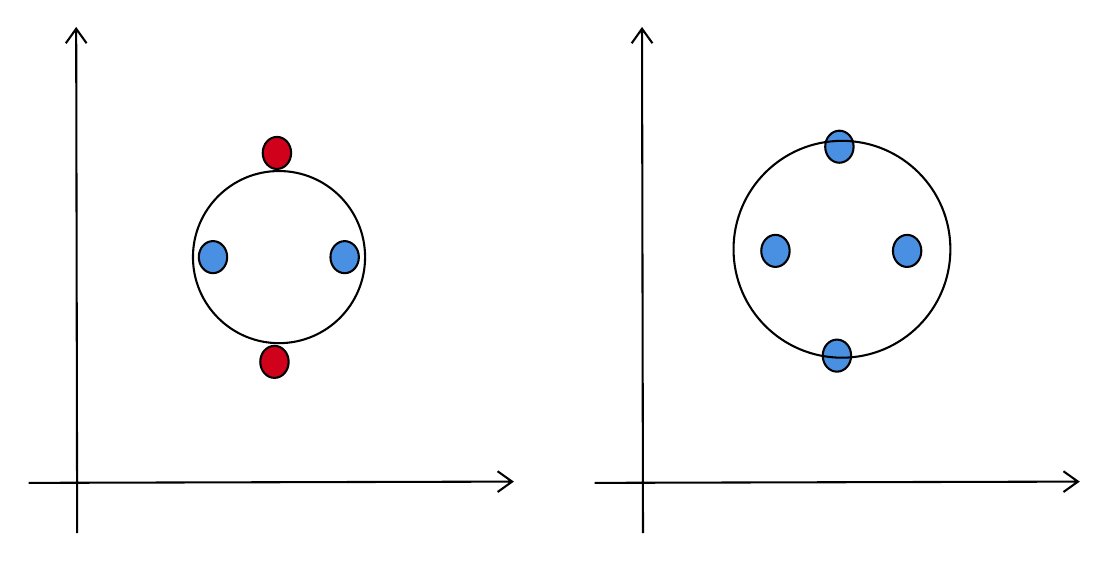
\begin{tikzpicture}[x=0.75pt,y=0.75pt,yscale=-1,xscale=1]
%uncomment if require: \path (0,414); %set diagram left start at 0, and has height of 414

%Shape: Ellipse [id:dp8126653472568731] 
\draw  [fill={rgb, 255:red, 208; green, 2; blue, 27 }  ,fill opacity=1 ] (170.67,142.4) .. controls (170.67,138.13) and (173.74,134.68) .. (177.51,134.68) .. controls (181.29,134.68) and (184.35,138.13) .. (184.35,142.4) .. controls (184.35,146.67) and (181.29,150.12) .. (177.51,150.12) .. controls (173.74,150.12) and (170.67,146.67) .. (170.67,142.4) -- cycle ;
%Shape: Ellipse [id:dp7933731782074234] 
\draw  [fill={rgb, 255:red, 74; green, 144; blue, 226 }  ,fill opacity=1 ] (139.86,192.59) .. controls (139.86,188.32) and (142.92,184.87) .. (146.7,184.87) .. controls (150.48,184.87) and (153.54,188.32) .. (153.54,192.59) .. controls (153.54,196.85) and (150.48,200.31) .. (146.7,200.31) .. controls (142.92,200.31) and (139.86,196.85) .. (139.86,192.59) -- cycle ;
%Shape: Ellipse [id:dp6470818868586241] 
\draw  [fill={rgb, 255:red, 74; green, 144; blue, 226 }  ,fill opacity=1 ] (203.3,192.62) .. controls (203.29,188.36) and (206.35,184.89) .. (210.12,184.88) .. controls (213.9,184.87) and (216.97,188.32) .. (216.98,192.59) .. controls (216.99,196.85) and (213.93,200.32) .. (210.15,200.33) .. controls (206.37,200.34) and (203.31,196.89) .. (203.3,192.62) -- cycle ;
%Shape: Ellipse [id:dp4572875498527885] 
\draw  [fill={rgb, 255:red, 208; green, 2; blue, 27 }  ,fill opacity=1 ] (169.48,243.07) .. controls (169.47,238.81) and (172.53,235.34) .. (176.31,235.33) .. controls (180.09,235.32) and (183.16,238.77) .. (183.16,243.04) .. controls (183.17,247.3) and (180.12,250.77) .. (176.34,250.78) .. controls (172.56,250.79) and (169.49,247.34) .. (169.48,243.07) -- cycle ;
%Shape: Circle [id:dp5458383365358183] 
\draw   (137.05,192.59) .. controls (137.05,169.69) and (155.61,151.12) .. (178.51,151.12) .. controls (201.42,151.12) and (219.98,169.69) .. (219.98,192.59) .. controls (219.98,215.49) and (201.42,234.05) .. (178.51,234.05) .. controls (155.61,234.05) and (137.05,215.49) .. (137.05,192.59) -- cycle ;

%Shape: Axis 2D [id:dp5790207644361977] 
\draw  (57.92,301.36) -- (290.83,300.75)(80.79,82.55) -- (81.26,325.6) (283.82,295.76) -- (290.83,300.75) -- (283.84,305.76) (75.8,89.56) -- (80.79,82.55) -- (85.8,89.54)  ;
%Shape: Axis 2D [id:dp8975872837595529] 
\draw  (330.54,301.36) -- (563.45,300.75)(353.41,82.55) -- (353.88,325.6) (556.44,295.76) -- (563.45,300.75) -- (556.46,305.76) (348.43,89.56) -- (353.41,82.55) -- (358.43,89.54)  ;
%Shape: Ellipse [id:dp42477847664701285] 
\draw  [fill={rgb, 255:red, 74; green, 144; blue, 226 }  ,fill opacity=1 ] (441.67,139.4) .. controls (441.67,135.13) and (444.74,131.68) .. (448.51,131.68) .. controls (452.29,131.68) and (455.35,135.13) .. (455.35,139.4) .. controls (455.35,143.67) and (452.29,147.12) .. (448.51,147.12) .. controls (444.74,147.12) and (441.67,143.67) .. (441.67,139.4) -- cycle ;
%Shape: Ellipse [id:dp9709173018884202] 
\draw  [fill={rgb, 255:red, 74; green, 144; blue, 226 }  ,fill opacity=1 ] (410.86,189.59) .. controls (410.86,185.32) and (413.92,181.87) .. (417.7,181.87) .. controls (421.48,181.87) and (424.54,185.32) .. (424.54,189.59) .. controls (424.54,193.85) and (421.48,197.31) .. (417.7,197.31) .. controls (413.92,197.31) and (410.86,193.85) .. (410.86,189.59) -- cycle ;
%Shape: Ellipse [id:dp4108028153688237] 
\draw  [fill={rgb, 255:red, 74; green, 144; blue, 226 }  ,fill opacity=1 ] (474.3,189.62) .. controls (474.29,185.36) and (477.35,181.89) .. (481.12,181.88) .. controls (484.9,181.87) and (487.97,185.32) .. (487.98,189.59) .. controls (487.99,193.85) and (484.93,197.32) .. (481.15,197.33) .. controls (477.37,197.34) and (474.31,193.89) .. (474.3,189.62) -- cycle ;
%Shape: Ellipse [id:dp08669361991465019] 
\draw  [fill={rgb, 255:red, 74; green, 144; blue, 226 }  ,fill opacity=1 ] (440.48,240.07) .. controls (440.47,235.81) and (443.53,232.34) .. (447.31,232.33) .. controls (451.09,232.32) and (454.16,235.77) .. (454.16,240.04) .. controls (454.17,244.3) and (451.12,247.77) .. (447.34,247.78) .. controls (443.56,247.79) and (440.49,244.34) .. (440.48,240.07) -- cycle ;
%Shape: Circle [id:dp12961460774468658] 
\draw   (397.5,188.81) .. controls (397.5,159.96) and (420.89,136.57) .. (449.74,136.57) .. controls (478.59,136.57) and (501.98,159.96) .. (501.98,188.81) .. controls (501.98,217.67) and (478.59,241.05) .. (449.74,241.05) .. controls (420.89,241.05) and (397.5,217.67) .. (397.5,188.81) -- cycle ;
\end{tikzpicture}\\

In the case of the tetragon, there will always be a combination of two points which are opposite of each other, with maximum distance among all points. These points can only be combined in a circle which has a diameter that is bigger or equal the distance between these two. By defintion, this circle will include the other points with lower distance.  

Since the VC dimension is the maximum number of points which can be shattered, the VC dimension of $\mathcal{A}$ is 3.\\

Now for the special case of all circles with radios one:

$$A _ { 1 } = \left\{ C _ { c , 1 } : c \in \mathbb { R } ^ { 2 } \right\}$$

Again, one and two points can be shattered without a problem. Further, three points can also be shattered, as long their arranged in a triangle that is inscribed in the unit circle. Further the points can't lie on the circle, but have to lie inside. It will be possible to shatter these three points as long as the sides of the triangle are sufficiently short. Again, for four points, the same issue arises as in the general case. So the VC dimension for unit circles in the plane is 3.

\section*{Shatter Coefficient of Half Spaces in $R^2$}

\subsection*{Half Spaces through the Origin}

First, we can determine the $n$-th shatter coefficient for the class of all half spaces containing the origin:

$$\mathcal { A } _ { 0 } = \left\{ H _ { a , b , 0 } : a , b \in \mathbb { R } \right\}$$ 

where 

$$H _ { a , b , c } = \left\{ ( x , y ) \in \mathbb { R } ^ { 2 } : a x + b y \geq c \right\}$$

In order to derive a general form of the shatter coefficient of $\mathcal{A}$ we need to establish a pattern of the shatter coefficient depending on the number of points. Clearly, one point can be either in or out of the set. Two points can be shattered in 4 sets. So up to $n=2$ the shatter coefficient is $2n$. In the case of three points, we can't shatter them anymore: \\

\tikzset{every picture/.style={line width=0.75pt}} %set default line width to 0.75pt        

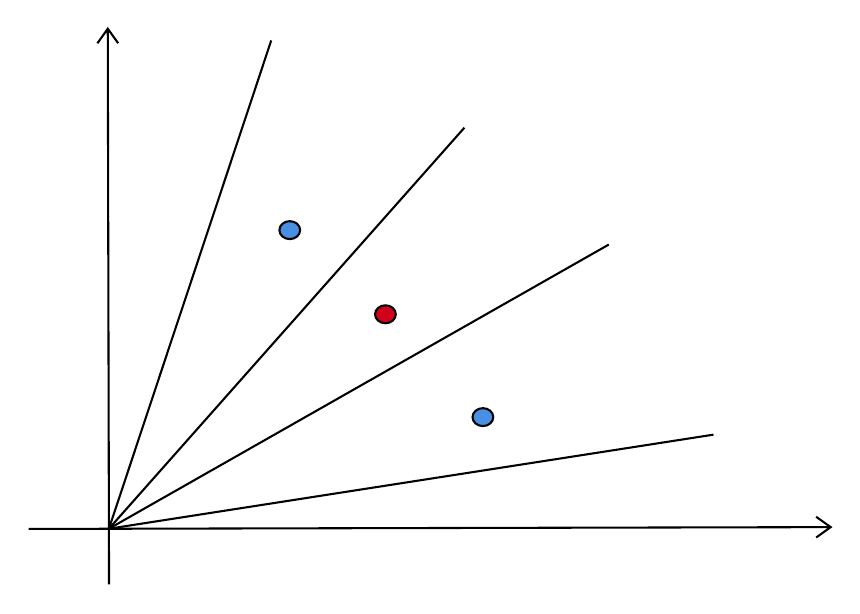
\begin{tikzpicture}[x=0.75pt,y=0.75pt,yscale=-1,xscale=1]
%uncomment if require: \path (0,419); %set diagram left start at 0, and has height of 419

%Shape: Axis 2D [id:dp5790207644361977] 
\draw  (27.05,255.24) -- (413.44,254.36)(65.14,14.23) -- (65.75,281.92) (406.43,249.37) -- (413.44,254.36) -- (406.45,259.37) (60.16,21.24) -- (65.14,14.23) -- (70.16,21.22)  ;
%Shape: Ellipse [id:dp8393226147780928] 
\draw  [fill={rgb, 255:red, 74; green, 144; blue, 226 }  ,fill opacity=1 ] (147.82,111.27) .. controls (147.82,108.89) and (150.06,106.95) .. (152.82,106.95) .. controls (155.58,106.95) and (157.82,108.89) .. (157.82,111.27) .. controls (157.82,113.66) and (155.58,115.59) .. (152.82,115.59) .. controls (150.06,115.59) and (147.82,113.66) .. (147.82,111.27) -- cycle ;
%Shape: Ellipse [id:dp6155363868313941] 
\draw  [fill={rgb, 255:red, 208; green, 2; blue, 27 }  ,fill opacity=1 ] (193.91,151.81) .. controls (193.91,149.43) and (196.15,147.49) .. (198.91,147.49) .. controls (201.67,147.49) and (203.91,149.43) .. (203.91,151.81) .. controls (203.91,154.2) and (201.67,156.13) .. (198.91,156.13) .. controls (196.15,156.13) and (193.91,154.2) .. (193.91,151.81) -- cycle ;
%Shape: Ellipse [id:dp2555721691736551] 
\draw  [fill={rgb, 255:red, 74; green, 144; blue, 226 }  ,fill opacity=1 ] (240.87,201.36) .. controls (240.87,198.98) and (243.11,197.04) .. (245.87,197.04) .. controls (248.63,197.04) and (250.87,198.98) .. (250.87,201.36) .. controls (250.87,203.74) and (248.63,205.68) .. (245.87,205.68) .. controls (243.11,205.68) and (240.87,203.74) .. (240.87,201.36) -- cycle ;
%Straight Lines [id:da6552617060200406] 
\draw    (65.68,255.14) -- (236.96,61.91) ;


%Straight Lines [id:da7962509781336733] 
\draw    (65.68,255.14) -- (306.53,118.22) ;


%Straight Lines [id:da7514812005108599] 
\draw    (65.68,255.14) -- (143.9,19.87) ;


%Straight Lines [id:da17953247410639328] 
\draw    (65.68,255.14) -- (356.97,209.81) ;

\end{tikzpicture} 
\newpage
More specifically, there is no set of points in which can shatter them into all possible sets containing two points, like seen above. So in this case the shatter coefficient will be 6, which is again $2n$. Any further point we add can either be in or out of a given set generated by a half space through the origin. So we can conclude, that the shatter coefficient of $\mathcal{A}_0$ in $R^2$ is 

$$S_{\mathcal{A}_0}(n) = 2n$$

\subsection*{General Half Spaces}

For establishing the nth-Shatter coefficient for general half spaces $\mathcal { A } = \left\{ H _ { a , b , c } : a , b , c \in \mathbb { R } \right\}$, we observe the following. Arranging all points on a circle in $R^2$,

\begin{itemize}
\item we can always generate sets containing all or none of the points using half-spaces, so the shatter coefficient will be at least two
\item it will always be possible to generate sets containing only one point, so the shatter coefficient will be at least 2 + n
\item it will be impossible to generate a set containing points opposite of each other without capturing adjacent points 
\item we can always group points together which are connected through the circle, as long as there is no point inbetween
\end{itemize}

The last observation leads us to the following result: There will always be a way for each point to be in a group of two, a group of three and so on, up to a group of $n-1$.   

\tikzset{every picture/.style={line width=0.75pt}} %set default line width to 0.75pt        

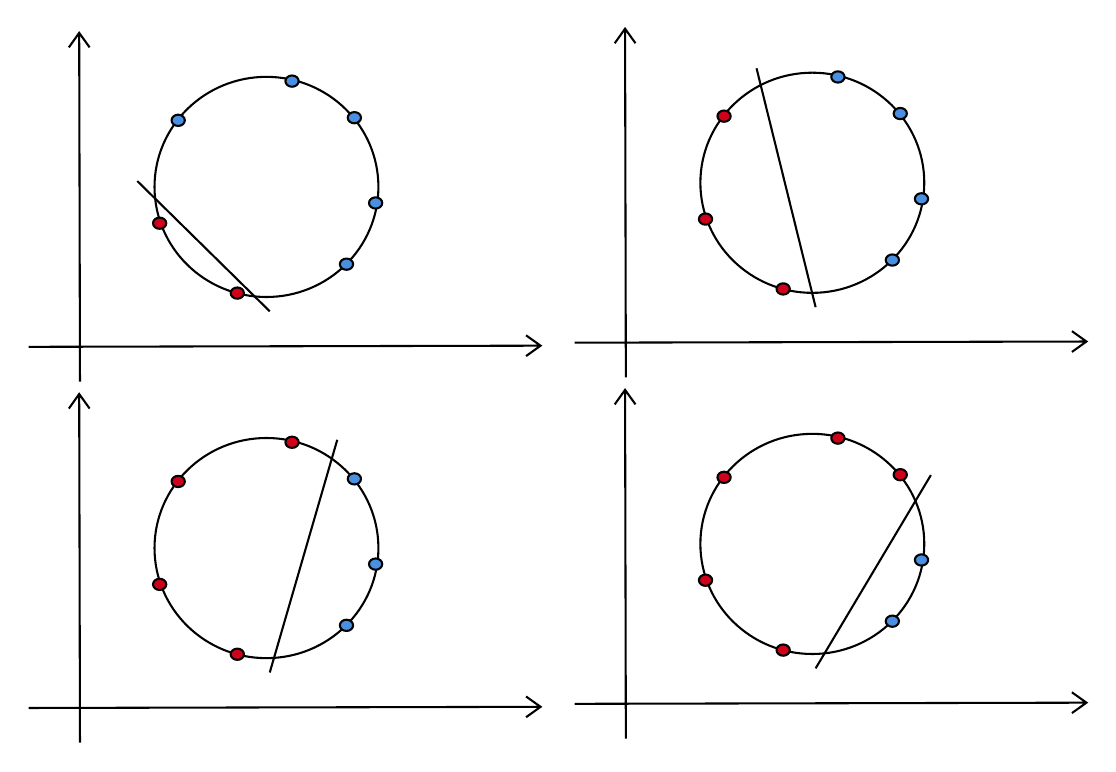
\begin{tikzpicture}[x=0.75pt,y=0.75pt,yscale=-1,xscale=1]
%uncomment if require: \path (0,419); %set diagram left start at 0, and has height of 419

%Shape: Ellipse [id:dp12680771317154427] 
\draw   (375.45,103.17) .. controls (375.45,73.88) and (399.6,50.13) .. (429.38,50.13) .. controls (459.17,50.13) and (483.32,73.88) .. (483.32,103.17) .. controls (483.32,132.46) and (459.17,156.2) .. (429.38,156.2) .. controls (399.6,156.2) and (375.45,132.46) .. (375.45,103.17) -- cycle ;
%Shape: Axis 2D [id:dp5790207644361977] 
\draw  (314.84,180.21) -- (561.46,179.65)(339.16,28.94) -- (339.54,196.95) (554.45,174.66) -- (561.46,179.65) -- (554.47,184.66) (334.18,35.95) -- (339.16,28.94) -- (344.18,35.93)  ;
%Shape: Ellipse [id:dp8393226147780928] 
\draw  [fill={rgb, 255:red, 74; green, 144; blue, 226 }  ,fill opacity=1 ] (438.52,52.19) .. controls (438.52,50.69) and (439.95,49.48) .. (441.71,49.48) .. controls (443.48,49.48) and (444.91,50.69) .. (444.91,52.19) .. controls (444.91,53.68) and (443.48,54.9) .. (441.71,54.9) .. controls (439.95,54.9) and (438.52,53.68) .. (438.52,52.19) -- cycle ;
%Shape: Ellipse [id:dp6155363868313941] 
\draw  [fill={rgb, 255:red, 74; green, 144; blue, 226 }  ,fill opacity=1 ] (478.79,110.89) .. controls (478.79,109.4) and (480.22,108.18) .. (481.98,108.18) .. controls (483.74,108.18) and (485.17,109.4) .. (485.17,110.89) .. controls (485.17,112.39) and (483.74,113.6) .. (481.98,113.6) .. controls (480.22,113.6) and (478.79,112.39) .. (478.79,110.89) -- cycle ;
%Shape: Ellipse [id:dp2555721691736551] 
\draw  [fill={rgb, 255:red, 74; green, 144; blue, 226 }  ,fill opacity=1 ] (468.55,69.82) .. controls (468.55,68.32) and (469.98,67.11) .. (471.75,67.11) .. controls (473.51,67.11) and (474.94,68.32) .. (474.94,69.82) .. controls (474.94,71.31) and (473.51,72.52) .. (471.75,72.52) .. controls (469.98,72.52) and (468.55,71.31) .. (468.55,69.82) -- cycle ;
%Shape: Ellipse [id:dp6057669435837836] 
\draw  [fill={rgb, 255:red, 74; green, 144; blue, 226 }  ,fill opacity=1 ] (464.75,140.39) .. controls (464.75,138.9) and (466.18,137.68) .. (467.94,137.68) .. controls (469.7,137.68) and (471.13,138.9) .. (471.13,140.39) .. controls (471.13,141.89) and (469.7,143.1) .. (467.94,143.1) .. controls (466.18,143.1) and (464.75,141.89) .. (464.75,140.39) -- cycle ;
%Shape: Ellipse [id:dp27101756834396573] 
\draw  [fill={rgb, 255:red, 208; green, 2; blue, 27 }  ,fill opacity=1 ] (412.15,154.32) .. controls (412.15,152.82) and (413.58,151.61) .. (415.34,151.61) .. controls (417.11,151.61) and (418.53,152.82) .. (418.53,154.32) .. controls (418.53,155.82) and (417.11,157.03) .. (415.34,157.03) .. controls (413.58,157.03) and (412.15,155.82) .. (412.15,154.32) -- cycle ;
%Shape: Ellipse [id:dp7676574036216017] 
\draw  [fill={rgb, 255:red, 208; green, 2; blue, 27 }  ,fill opacity=1 ] (383.67,71.07) .. controls (383.67,69.57) and (385.1,68.36) .. (386.86,68.36) .. controls (388.62,68.36) and (390.05,69.57) .. (390.05,71.07) .. controls (390.05,72.57) and (388.62,73.78) .. (386.86,73.78) .. controls (385.1,73.78) and (383.67,72.57) .. (383.67,71.07) -- cycle ;
%Shape: Ellipse [id:dp4860988989330426] 
\draw  [fill={rgb, 255:red, 208; green, 2; blue, 27 }  ,fill opacity=1 ] (374.73,120.65) .. controls (374.73,119.16) and (376.16,117.94) .. (377.92,117.94) .. controls (379.69,117.94) and (381.12,119.16) .. (381.12,120.65) .. controls (381.12,122.15) and (379.69,123.36) .. (377.92,123.36) .. controls (376.16,123.36) and (374.73,122.15) .. (374.73,120.65) -- cycle ;
%Straight Lines [id:da6403664120681241] 
\draw    (402.5,48) -- (430.98,163.11) ;


%Shape: Ellipse [id:dp3734180149763112] 
\draw   (112.45,105.17) .. controls (112.45,75.88) and (136.6,52.13) .. (166.38,52.13) .. controls (196.17,52.13) and (220.32,75.88) .. (220.32,105.17) .. controls (220.32,134.46) and (196.17,158.2) .. (166.38,158.2) .. controls (136.6,158.2) and (112.45,134.46) .. (112.45,105.17) -- cycle ;
%Shape: Axis 2D [id:dp9369936214640792] 
\draw  (51.84,182.21) -- (298.46,181.65)(76.16,30.94) -- (76.54,198.95) (291.45,176.66) -- (298.46,181.65) -- (291.47,186.66) (71.18,37.95) -- (76.16,30.94) -- (81.18,37.93)  ;
%Shape: Ellipse [id:dp8511383587464889] 
\draw  [fill={rgb, 255:red, 74; green, 144; blue, 226 }  ,fill opacity=1 ] (175.52,54.19) .. controls (175.52,52.69) and (176.95,51.48) .. (178.71,51.48) .. controls (180.48,51.48) and (181.91,52.69) .. (181.91,54.19) .. controls (181.91,55.68) and (180.48,56.9) .. (178.71,56.9) .. controls (176.95,56.9) and (175.52,55.68) .. (175.52,54.19) -- cycle ;
%Shape: Ellipse [id:dp21386979622118973] 
\draw  [fill={rgb, 255:red, 74; green, 144; blue, 226 }  ,fill opacity=1 ] (215.79,112.89) .. controls (215.79,111.4) and (217.22,110.18) .. (218.98,110.18) .. controls (220.74,110.18) and (222.17,111.4) .. (222.17,112.89) .. controls (222.17,114.39) and (220.74,115.6) .. (218.98,115.6) .. controls (217.22,115.6) and (215.79,114.39) .. (215.79,112.89) -- cycle ;
%Shape: Ellipse [id:dp7641006442084969] 
\draw  [fill={rgb, 255:red, 74; green, 144; blue, 226 }  ,fill opacity=1 ] (205.55,71.82) .. controls (205.55,70.32) and (206.98,69.11) .. (208.75,69.11) .. controls (210.51,69.11) and (211.94,70.32) .. (211.94,71.82) .. controls (211.94,73.31) and (210.51,74.52) .. (208.75,74.52) .. controls (206.98,74.52) and (205.55,73.31) .. (205.55,71.82) -- cycle ;
%Shape: Ellipse [id:dp6850843972569106] 
\draw  [fill={rgb, 255:red, 74; green, 144; blue, 226 }  ,fill opacity=1 ] (201.75,142.39) .. controls (201.75,140.9) and (203.18,139.68) .. (204.94,139.68) .. controls (206.7,139.68) and (208.13,140.9) .. (208.13,142.39) .. controls (208.13,143.89) and (206.7,145.1) .. (204.94,145.1) .. controls (203.18,145.1) and (201.75,143.89) .. (201.75,142.39) -- cycle ;
%Shape: Ellipse [id:dp1158866223725451] 
\draw  [fill={rgb, 255:red, 208; green, 2; blue, 27 }  ,fill opacity=1 ] (149.15,156.32) .. controls (149.15,154.82) and (150.58,153.61) .. (152.34,153.61) .. controls (154.11,153.61) and (155.53,154.82) .. (155.53,156.32) .. controls (155.53,157.82) and (154.11,159.03) .. (152.34,159.03) .. controls (150.58,159.03) and (149.15,157.82) .. (149.15,156.32) -- cycle ;
%Shape: Ellipse [id:dp9484484829855445] 
\draw  [fill={rgb, 255:red, 74; green, 144; blue, 226 }  ,fill opacity=1 ] (120.67,73.07) .. controls (120.67,71.57) and (122.1,70.36) .. (123.86,70.36) .. controls (125.62,70.36) and (127.05,71.57) .. (127.05,73.07) .. controls (127.05,74.57) and (125.62,75.78) .. (123.86,75.78) .. controls (122.1,75.78) and (120.67,74.57) .. (120.67,73.07) -- cycle ;
%Shape: Ellipse [id:dp4146557196560683] 
\draw  [fill={rgb, 255:red, 208; green, 2; blue, 27 }  ,fill opacity=1 ] (111.73,122.65) .. controls (111.73,121.16) and (113.16,119.94) .. (114.92,119.94) .. controls (116.69,119.94) and (118.12,121.16) .. (118.12,122.65) .. controls (118.12,124.15) and (116.69,125.36) .. (114.92,125.36) .. controls (113.16,125.36) and (111.73,124.15) .. (111.73,122.65) -- cycle ;
%Straight Lines [id:da9351269251852833] 
\draw    (104.16,102.34) -- (167.98,165.11) ;



%Shape: Ellipse [id:dp2995916334033466] 
\draw   (375.45,277.17) .. controls (375.45,247.88) and (399.6,224.13) .. (429.38,224.13) .. controls (459.17,224.13) and (483.32,247.88) .. (483.32,277.17) .. controls (483.32,306.46) and (459.17,330.2) .. (429.38,330.2) .. controls (399.6,330.2) and (375.45,306.46) .. (375.45,277.17) -- cycle ;
%Shape: Axis 2D [id:dp31316304718979016] 
\draw  (314.84,354.21) -- (561.46,353.65)(339.16,202.94) -- (339.54,370.95) (554.45,348.66) -- (561.46,353.65) -- (554.47,358.66) (334.18,209.95) -- (339.16,202.94) -- (344.18,209.93)  ;
%Shape: Ellipse [id:dp6030000097224409] 
\draw  [fill={rgb, 255:red, 208; green, 2; blue, 27 }  ,fill opacity=1 ] (438.52,226.19) .. controls (438.52,224.69) and (439.95,223.48) .. (441.71,223.48) .. controls (443.48,223.48) and (444.91,224.69) .. (444.91,226.19) .. controls (444.91,227.68) and (443.48,228.9) .. (441.71,228.9) .. controls (439.95,228.9) and (438.52,227.68) .. (438.52,226.19) -- cycle ;
%Shape: Ellipse [id:dp5327308224791552] 
\draw  [fill={rgb, 255:red, 74; green, 144; blue, 226 }  ,fill opacity=1 ] (478.79,284.89) .. controls (478.79,283.4) and (480.22,282.18) .. (481.98,282.18) .. controls (483.74,282.18) and (485.17,283.4) .. (485.17,284.89) .. controls (485.17,286.39) and (483.74,287.6) .. (481.98,287.6) .. controls (480.22,287.6) and (478.79,286.39) .. (478.79,284.89) -- cycle ;
%Shape: Ellipse [id:dp22920013150948393] 
\draw  [fill={rgb, 255:red, 208; green, 2; blue, 27 }  ,fill opacity=1 ] (468.55,243.82) .. controls (468.55,242.32) and (469.98,241.11) .. (471.75,241.11) .. controls (473.51,241.11) and (474.94,242.32) .. (474.94,243.82) .. controls (474.94,245.31) and (473.51,246.52) .. (471.75,246.52) .. controls (469.98,246.52) and (468.55,245.31) .. (468.55,243.82) -- cycle ;
%Shape: Ellipse [id:dp7064584533733218] 
\draw  [fill={rgb, 255:red, 74; green, 144; blue, 226 }  ,fill opacity=1 ] (464.75,314.39) .. controls (464.75,312.9) and (466.18,311.68) .. (467.94,311.68) .. controls (469.7,311.68) and (471.13,312.9) .. (471.13,314.39) .. controls (471.13,315.89) and (469.7,317.1) .. (467.94,317.1) .. controls (466.18,317.1) and (464.75,315.89) .. (464.75,314.39) -- cycle ;
%Shape: Ellipse [id:dp5493384876284498] 
\draw  [fill={rgb, 255:red, 208; green, 2; blue, 27 }  ,fill opacity=1 ] (412.15,328.32) .. controls (412.15,326.82) and (413.58,325.61) .. (415.34,325.61) .. controls (417.11,325.61) and (418.53,326.82) .. (418.53,328.32) .. controls (418.53,329.82) and (417.11,331.03) .. (415.34,331.03) .. controls (413.58,331.03) and (412.15,329.82) .. (412.15,328.32) -- cycle ;
%Shape: Ellipse [id:dp9474589982695697] 
\draw  [fill={rgb, 255:red, 208; green, 2; blue, 27 }  ,fill opacity=1 ] (383.67,245.07) .. controls (383.67,243.57) and (385.1,242.36) .. (386.86,242.36) .. controls (388.62,242.36) and (390.05,243.57) .. (390.05,245.07) .. controls (390.05,246.57) and (388.62,247.78) .. (386.86,247.78) .. controls (385.1,247.78) and (383.67,246.57) .. (383.67,245.07) -- cycle ;
%Shape: Ellipse [id:dp1625929682771866] 
\draw  [fill={rgb, 255:red, 208; green, 2; blue, 27 }  ,fill opacity=1 ] (374.73,294.65) .. controls (374.73,293.16) and (376.16,291.94) .. (377.92,291.94) .. controls (379.69,291.94) and (381.12,293.16) .. (381.12,294.65) .. controls (381.12,296.15) and (379.69,297.36) .. (377.92,297.36) .. controls (376.16,297.36) and (374.73,296.15) .. (374.73,294.65) -- cycle ;
%Straight Lines [id:da33495925766079404] 
\draw    (486.5,244) -- (430.98,337.11) ;


%Shape: Ellipse [id:dp9102471797678306] 
\draw   (112.45,279.17) .. controls (112.45,249.88) and (136.6,226.13) .. (166.38,226.13) .. controls (196.17,226.13) and (220.32,249.88) .. (220.32,279.17) .. controls (220.32,308.46) and (196.17,332.2) .. (166.38,332.2) .. controls (136.6,332.2) and (112.45,308.46) .. (112.45,279.17) -- cycle ;
%Shape: Axis 2D [id:dp9357135264408839] 
\draw  (51.84,356.21) -- (298.46,355.65)(76.16,204.94) -- (76.54,372.95) (291.45,350.66) -- (298.46,355.65) -- (291.47,360.66) (71.18,211.95) -- (76.16,204.94) -- (81.18,211.93)  ;
%Shape: Ellipse [id:dp8675073308978304] 
\draw  [fill={rgb, 255:red, 208; green, 2; blue, 27 }  ,fill opacity=1 ] (175.52,228.19) .. controls (175.52,226.69) and (176.95,225.48) .. (178.71,225.48) .. controls (180.48,225.48) and (181.91,226.69) .. (181.91,228.19) .. controls (181.91,229.68) and (180.48,230.9) .. (178.71,230.9) .. controls (176.95,230.9) and (175.52,229.68) .. (175.52,228.19) -- cycle ;
%Shape: Ellipse [id:dp9620263531172891] 
\draw  [fill={rgb, 255:red, 74; green, 144; blue, 226 }  ,fill opacity=1 ] (215.79,286.89) .. controls (215.79,285.4) and (217.22,284.18) .. (218.98,284.18) .. controls (220.74,284.18) and (222.17,285.4) .. (222.17,286.89) .. controls (222.17,288.39) and (220.74,289.6) .. (218.98,289.6) .. controls (217.22,289.6) and (215.79,288.39) .. (215.79,286.89) -- cycle ;
%Shape: Ellipse [id:dp2926912846954729] 
\draw  [fill={rgb, 255:red, 74; green, 144; blue, 226 }  ,fill opacity=1 ] (205.55,245.82) .. controls (205.55,244.32) and (206.98,243.11) .. (208.75,243.11) .. controls (210.51,243.11) and (211.94,244.32) .. (211.94,245.82) .. controls (211.94,247.31) and (210.51,248.52) .. (208.75,248.52) .. controls (206.98,248.52) and (205.55,247.31) .. (205.55,245.82) -- cycle ;
%Shape: Ellipse [id:dp932800030523898] 
\draw  [fill={rgb, 255:red, 74; green, 144; blue, 226 }  ,fill opacity=1 ] (201.75,316.39) .. controls (201.75,314.9) and (203.18,313.68) .. (204.94,313.68) .. controls (206.7,313.68) and (208.13,314.9) .. (208.13,316.39) .. controls (208.13,317.89) and (206.7,319.1) .. (204.94,319.1) .. controls (203.18,319.1) and (201.75,317.89) .. (201.75,316.39) -- cycle ;
%Shape: Ellipse [id:dp4771597212632983] 
\draw  [fill={rgb, 255:red, 208; green, 2; blue, 27 }  ,fill opacity=1 ] (149.15,330.32) .. controls (149.15,328.82) and (150.58,327.61) .. (152.34,327.61) .. controls (154.11,327.61) and (155.53,328.82) .. (155.53,330.32) .. controls (155.53,331.82) and (154.11,333.03) .. (152.34,333.03) .. controls (150.58,333.03) and (149.15,331.82) .. (149.15,330.32) -- cycle ;
%Shape: Ellipse [id:dp8745673004467913] 
\draw  [fill={rgb, 255:red, 208; green, 2; blue, 27 }  ,fill opacity=1 ] (120.67,247.07) .. controls (120.67,245.57) and (122.1,244.36) .. (123.86,244.36) .. controls (125.62,244.36) and (127.05,245.57) .. (127.05,247.07) .. controls (127.05,248.57) and (125.62,249.78) .. (123.86,249.78) .. controls (122.1,249.78) and (120.67,248.57) .. (120.67,247.07) -- cycle ;
%Shape: Ellipse [id:dp29072350495528043] 
\draw  [fill={rgb, 255:red, 208; green, 2; blue, 27 }  ,fill opacity=1 ] (111.73,296.65) .. controls (111.73,295.16) and (113.16,293.94) .. (114.92,293.94) .. controls (116.69,293.94) and (118.12,295.16) .. (118.12,296.65) .. controls (118.12,298.15) and (116.69,299.36) .. (114.92,299.36) .. controls (113.16,299.36) and (111.73,298.15) .. (111.73,296.65) -- cycle ;
%Straight Lines [id:da6793375976424423] 
\draw    (200.5,227) -- (167.98,339.11) ;

\end{tikzpicture}

Consequently, the shatter coefficient for the group of all half-spaces will be: 

$$S _ { \mathcal { A } } ( n ) = 2+ n(n-1)$$


\section*{Rademacher Averages}

\subsubsection*{First Structural Result}

\begin{align*}
R _ { n } ( A \cup B ) &= \mathbf { E } \sup _ { x \in A \cup B  } \frac { 1 } { n } \left| \sum _ { i = 1 } ^ { n } \sigma _ { i } x _ { i } \right| \\
&\leq \mathbf { E } \sup _ { a \in A } \frac { 1 } { n } \left| \sum _ { i = 1 } ^ { n } \sigma _ { i } a _ { i } \right| + \mathbf { E } \sup _ { b \in B } \frac { 1 } { n } \left| \sum _ { i = 1 } ^ { n } \sigma _ { i } b _ { i } \right| \\
&= R _ { n } ( A ) + R _ { n } ( B )
\end{align*}

\subsubsection*{Second Structural Result}
Note, that $c$ is a constant.

\begin{align*}
R _ { n } (cA ) &=  \mathbf { E } \sup _ { a \in A } \frac { 1 } { n } \left| \sum _ { i = 1 } ^ { n } \sigma _ { i } c \cdot a _ { i } \right| \\
&=\mathbf { E } \sup _ { a \in A }  |c| \cdot \frac { 1 } { n } \left| \sum _ { i = 1 } ^ { n } \sigma _ { i } a _ { i } \right| \\
&= |c| \cdot \mathbf { E } \sup _ { a \in A }  \frac { 1 } { n } \left| \sum _ { i = 1 } ^ { n } \sigma _ { i } a _ { i } \right| \\
&= |c| \cdot R _ { n } ( A )
\end{align*}

\subsubsection*{Third Structural Result}

\begin{align*}
R _ { n } ( A \oplus B ) &= \mathbb { E } \sup _ { a \in \mathcal { A } , b \in \mathcal { B } } \left| \frac { 1 } { n } \sum _ { i = 1 } ^ { n } \sigma _ { i } \left( a _ { i } + b _ { i } \right) \right| \\
&\leq \mathbb { E } \sup _ { a \in \mathcal { A } } \left| \frac { 1 } { n } \sum _ { i = 1 } ^ { n } \sigma _ { i } a _ { i } \right| + \underset { b \in \mathcal { B } } { \operatorname { E } \sup } \left| \frac { 1 } { n } \sum _ { i = 1 } ^ { n } \sigma _ { i } b _ { i } \right| \\
&= R _ { n } ( \mathcal { A } ) + R _ { n } ( \mathcal { B } )
\end{align*}

The second step uses the triangle inequality applied to the supremum.

\subsubsection*{Fourth Structural Result}

For the last result we can make use of the previous ones. 

First we note that the absolute convex hull of $\mathcal{A}$ contains the set itself. 

$$\mathcal { A } \subset \text {absconv} (\mathcal { A })$$

therefore $R _ { n } ( \mathcal { A } ) \leq R _ { n } ( \text { absconv } \mathcal { A } )$

Where $\operatorname { absconv } ( A ) = \left\{ \sum _ { j = 1 } ^ { N } c _ { j } a ^ { ( j ) } : N \in \mathbb { N } , \sum _ { j = 1 } ^ { N } \left| c _ { j } \right| \leq 1 , a ^ { ( j ) } \in A \right\}$ \\

Further, for any value of $c_j$ we have 
$$R _ { n } \left( c _ { 1 } \mathcal { A } + \ldots + c _ { N } \mathcal { A } \right) \leq \sum _ { i = 1 } ^ { N } \left| c _ { i } \right| R _ { n } ( \mathcal { A } ) \leq R _ { n } ( \mathcal { A } )$$

where $\sum _ { j = 1 } ^ { N } \left| c _ { j } \right| = 1$. Since the absolute convex hull is the union of all sets of the form

$$c _ { 1 } \mathcal { A } + \ldots + c _ { N } \mathcal { A } \equiv \left\{ c _ { 1 } a _ { 1 } + \ldots + c _ { N } a _ { N } : a _ { 1 } , \ldots , a _ { N } \in \mathcal { A } \right\}$$

Consequently, $R _ { n } ( \mathcal { A } ) = R _ { n } ($absconv$(\mathcal { A }) )$.


\section*{The Perceptron Algorithm}

\subsubsection*{Linearly Seperable Data}

As we noted in class, the perceptron algorithm is guaranteed to converge with linearly seperable data. Further, we derived that the algorithm will run for a maximum of $\frac{R^2}{\gamma^2}$ rounds where $R = \max ||x||$ and $\gamma$ denotes the margin.

\begin{figure}[H]
\centering
Convergence and Empirical Risk in $R^2$
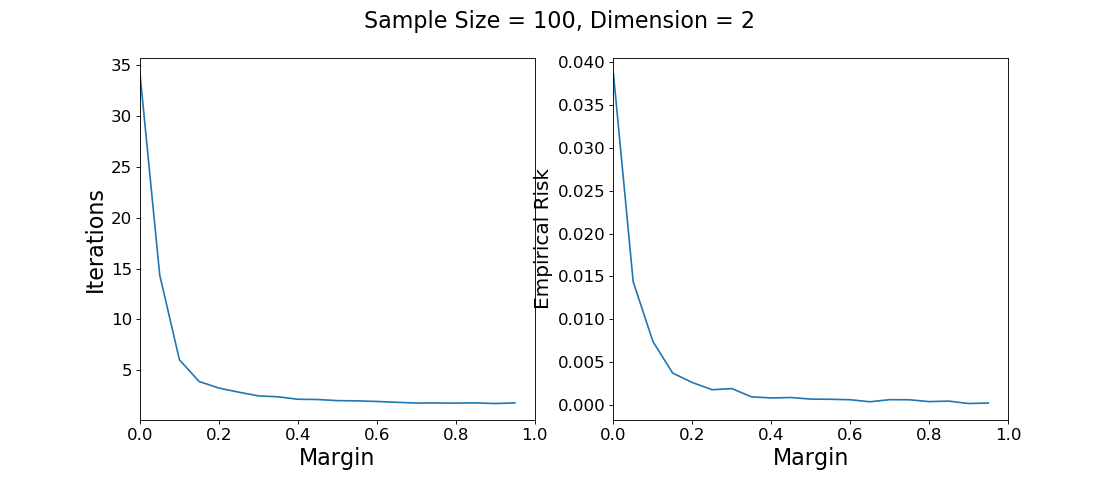
\includegraphics[scale= 0.4]{Perceptron_Seperable100_d2}
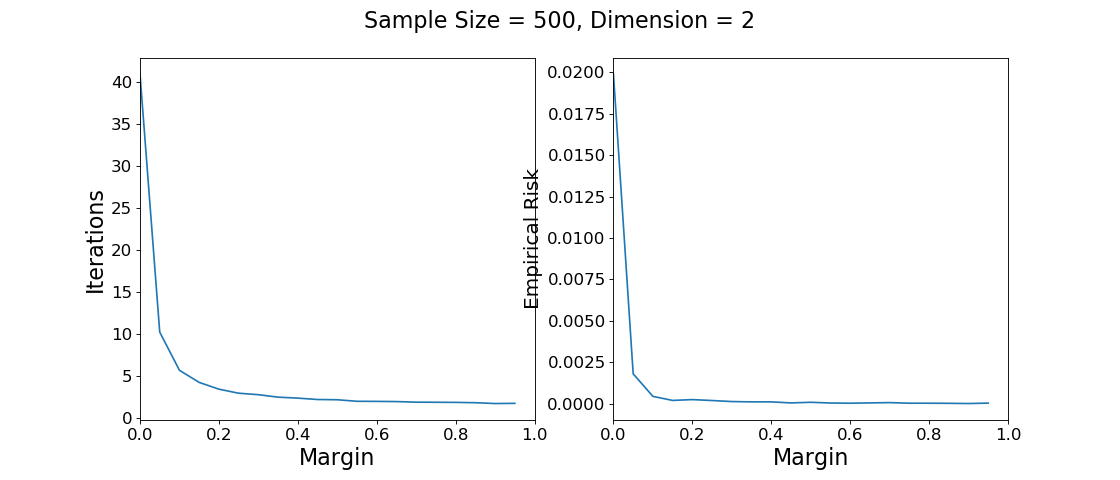
\includegraphics[scale= 0.4]{Perceptron_Seperable500_d2}
\end{figure}

The simulations show, that the algorithm converges quickly in $R^2$ even for margins below 0.2. Further, the estimated probability of error is close to zero, once the margin exceeds 0.1. 
The sample size doesn't influence the number of iterations. Larger samples improve the empirical risk for lower margins. 


For higher dimensional spaces we have a similar picture, however with a higher number of iterations and empirical risk.

\begin{figure}[H]
\centering
Convergence and Empirical Risk in $R^{10}$
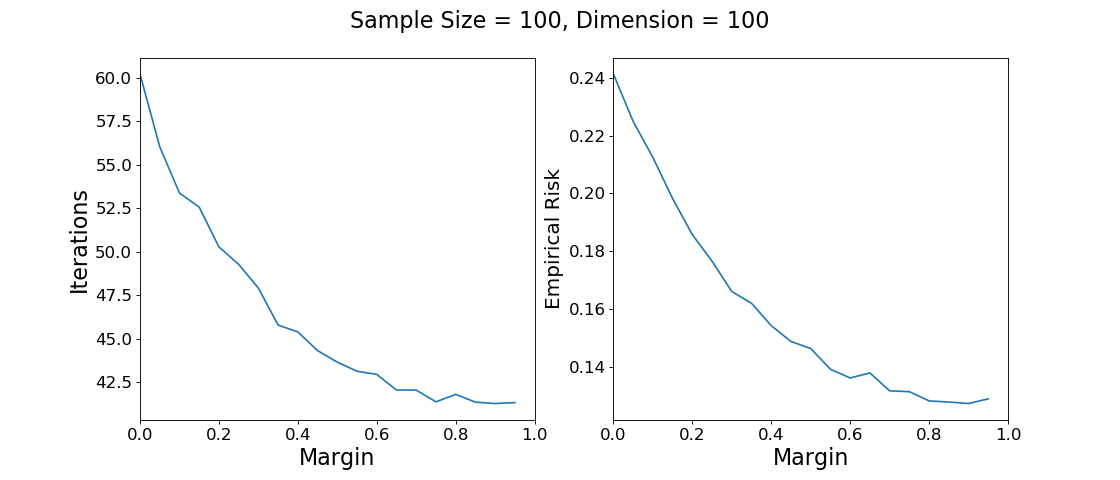
\includegraphics[scale= 0.4]{Perceptron_Seperable100_d100}
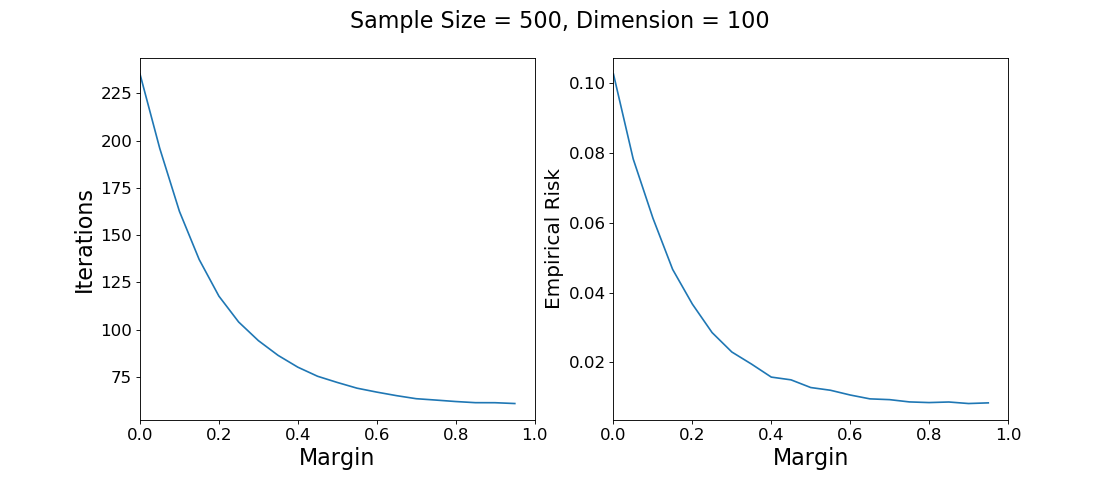
\includegraphics[scale= 0.4]{Perceptron_Seperable500_d100}
\end{figure}

Again, as the margin increases the number of iterations falls. However, the overall number of iterations in $R^{10}$ is much higher than in $R^2$, for the same margins. Why is that so? Since we keep $\gamma$ constant, we need to find bounds for the maximum norm $R$. In the worst case scenario we have one observation which has all entries either 1 or $-1$ (depending on the class). In that case the maximum norm would be $\sqrt{\sum_{i=1}^d x_i^2} = \sqrt{d}$. So the upper bound for the number of iterations will be $d/\gamma$. We can clearly see in the simulations, that the perceptron stays below this bound, even for larger margins. The sample size seems to play a role for larger samples, probably since the chances of having higher $R$ values increases. Finally, the probability of error converges to zero, but slower than in the two dimensional case.
\newpage
\subsubsection*{Non-Seperable Case}

For the non-seperable case we need to include a stopping condition. The condition used in my simulation is a maximum number of iterations of 2000 or the in-sample accuracy doesn't change more than by $10^{-5}$. Further, without centering and re-scaling the input data the perceptron algorithm will perform badly, as shown in the following plot:

\begin{figure*}[htp]
    \centering
    \begin{subfigure}{0.5\textwidth}
      \centering
      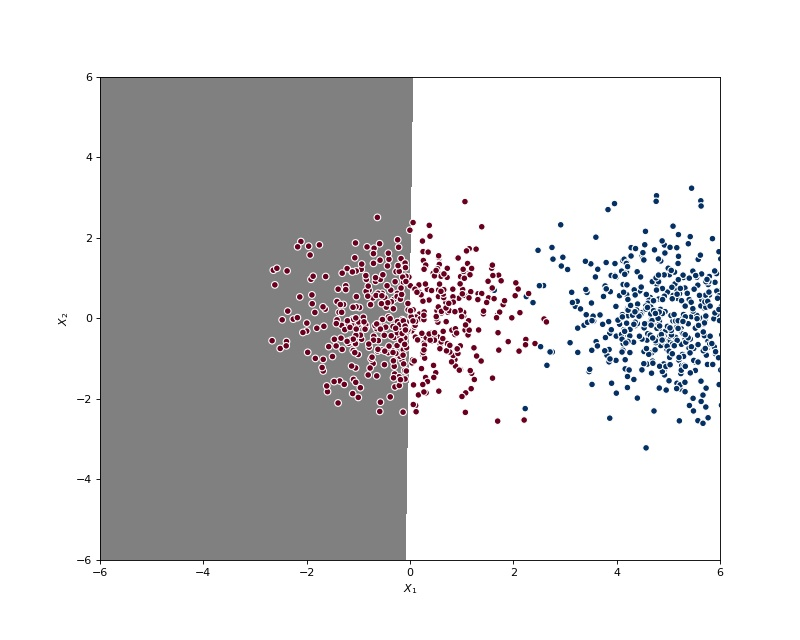
\includegraphics[scale= 0.25]{R2_Convergence/Perceptron_NOSCALE_round_32}
      \caption{}
    \end{subfigure}%
    \begin{subfigure}{0.5\textwidth}
      \centering
      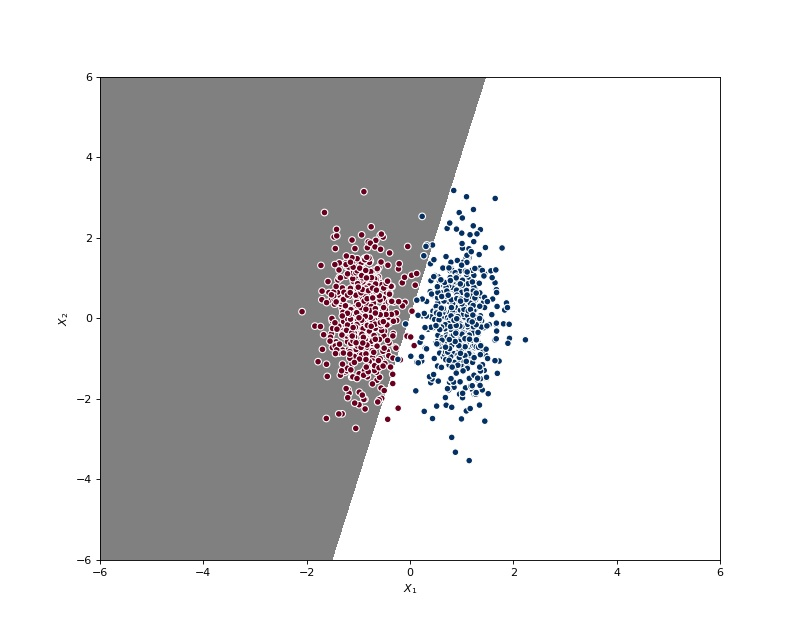
\includegraphics[scale= 0.25]{R2_Convergence/Perceptron_SCALE_round_30}
      \caption{}
    \end{subfigure}
  \caption { (a) No Scaling (b) Scaling}
\end{figure*}

\textbf{Bayes Risk} \\
The Bayes classifier $g^*$ predicts 1 if $\eta(x) \geq 0.5$ and -1 else, with $\eta(x) = f_{Y=1|X}$.
We can visualize the error region of the Bayes classifier graphically:

\begin{figure}[H]
\centering
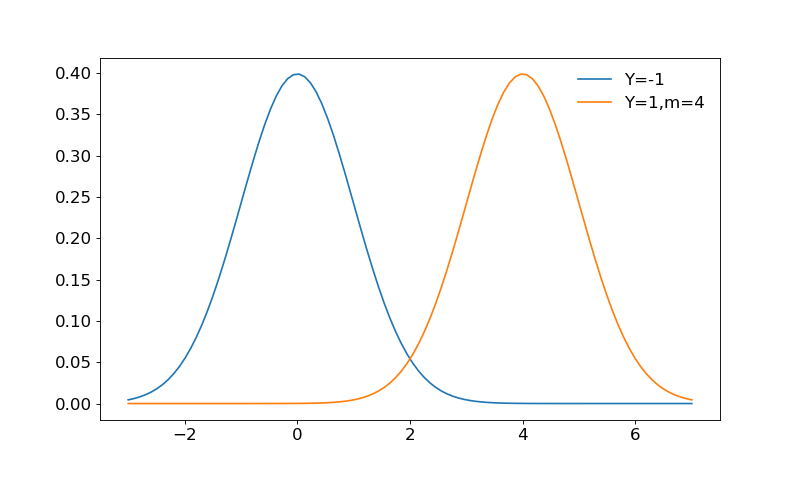
\includegraphics[scale= 0.4]{Bayes_Risk}
\end{figure}

The error region is indicated by the overlap of the two conditional density functions. 
The expected loss is:

$$E\left[l(g,y) \right] = \mathbb{1}_{g=1} P(Y=-1 |X < m/2) + \mathbb{1}_{g=-1} P(Y= 1 | X >m/2)$$

Which leads to a Bayes risk of 

$$R(g^*) = \Phi\left(m/2 \right)$$

with $\Phi$ being the CDF of the normal distribution with mean $m$ and variance one. 

\textbf{Results}\\
Once the data is scaled, the empirical risk convergec towards zero with larger seperation between the two clusters (indicated by $m$).The number of iterations for low seperation is considerably higher than the iterations in the seperable case. However, as the distance between the clusters increases, the sample data becomes linearly seperable and the algorithm converges quickly. 

\begin{figure}[H]
\centering
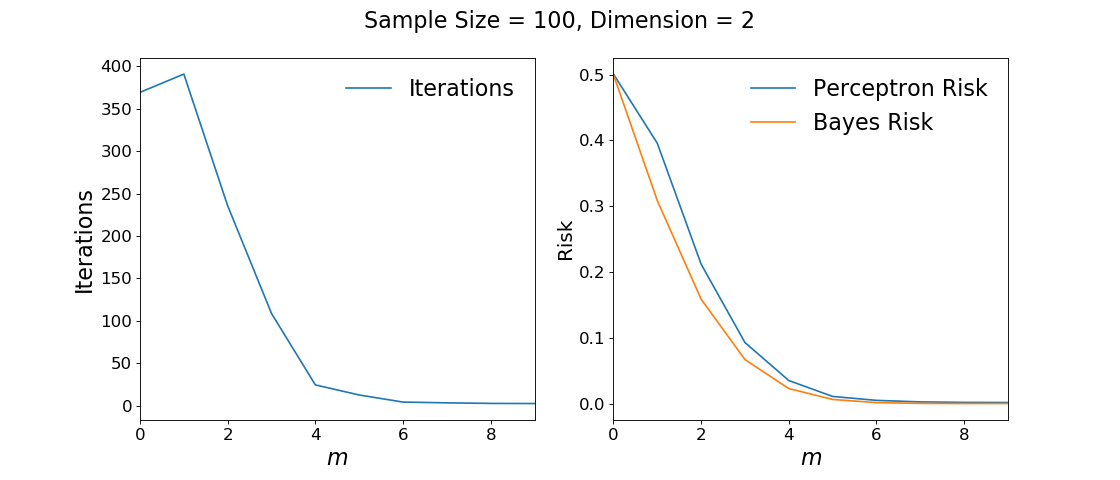
\includegraphics[scale= 0.4]{Perceptron_Non_Seperable100_d2}
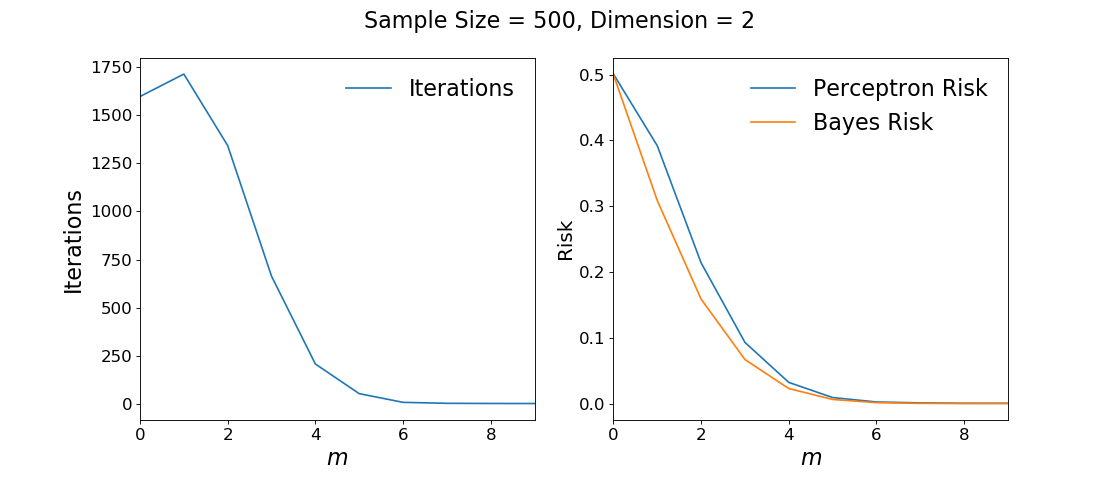
\includegraphics[scale= 0.4]{Perceptron_Non_Seperable500_d2}
\end{figure}

For larger samples, the algorithm reaches its stopping condition less quickly, while the empirical risk seems similar. Overall, the empirical risk converges towards zero with larger values of $m$. However, without scaling, the empirical risk will converge towards a value of 0.25. 
\newpage

We can find similar results for higher-dimensional data. Larger sample sizes have a positive influence on the risk, but also lead to a higher number of iterations. 

\begin{figure}[H]
\centering
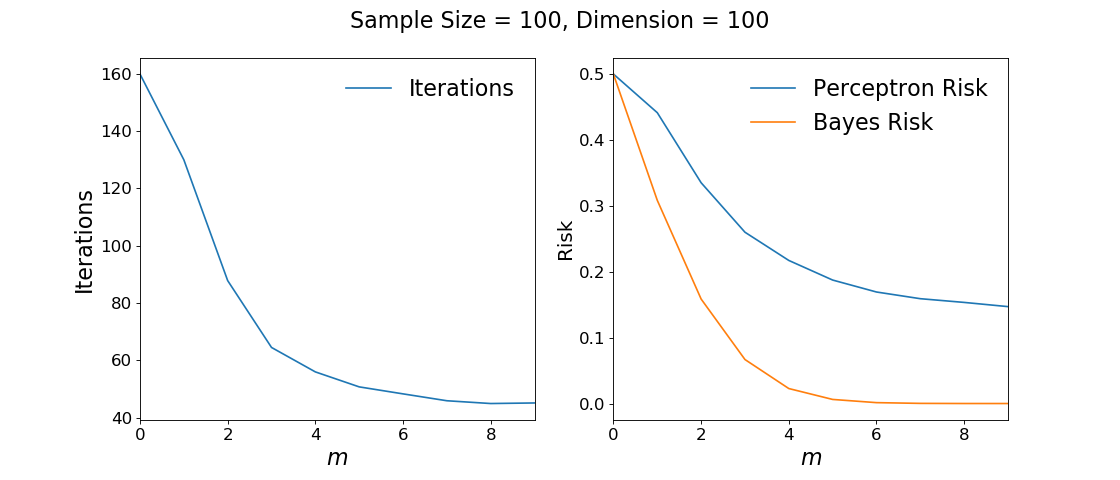
\includegraphics[scale= 0.4]{Perceptron_Non_Seperable100_d100}
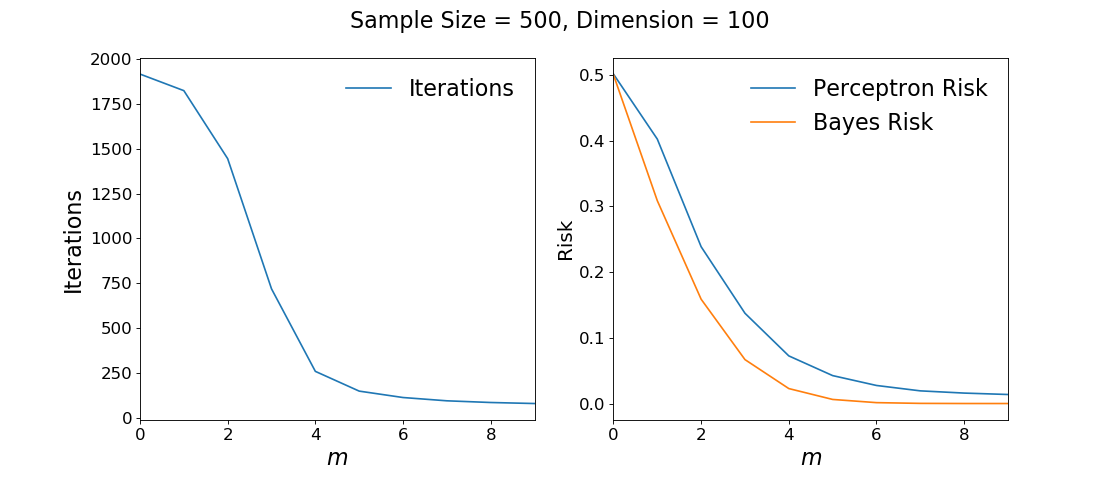
\includegraphics[scale= 0.4]{Perceptron_Non_Seperable500_d100}
\end{figure}

\end{document}


 